% ============================================================
%  Reporte Final — Proyecto de IA  TC3002B
%  Dataset: Spotify Tracks (Kaggle / Maharshi Pandya)
% ============================================================
\documentclass[12pt,a4paper]{article}

\usepackage[utf8]{inputenc}
\usepackage[T1]{fontenc}
\usepackage{lmodern}
\usepackage{geometry}
\geometry{top=2.5cm, bottom=2.5cm, left=2.8cm, right=2.8cm}
\usepackage{graphicx}
\usepackage{booktabs}
\usepackage{array}
\usepackage{amsmath}
\usepackage{amssymb}
\usepackage{float}
\usepackage{caption}
\usepackage{subcaption}
\usepackage{xcolor}
\usepackage[hidelinks]{hyperref}
\usepackage{enumitem}
\usepackage{parskip}
\usepackage{tcolorbox}
\usepackage{tikz}
\usetikzlibrary{positioning,arrows.meta,shapes.geometric,matrix,calc,decorations.pathreplacing}

% ---------- Colores ---------------------------------------------------
\definecolor{spotgreen}{HTML}{1DB954}
\definecolor{spotdark}{HTML}{191414}
\definecolor{spotgray}{HTML}{535353}
\definecolor{accentblue}{HTML}{2563EB}
\definecolor{warnred}{HTML}{DC2626}
\definecolor{lightgray}{HTML}{F3F4F6}

% ---------- Cajas especiales ------------------------------------------
\tcbuselibrary{breakable}

\newtcolorbox{ejecutivo}{
  colback=spotgreen!8,
  colframe=spotgreen!60!black,
  fonttitle=\bfseries\small,
  title=Conclusi\'on Ejecutiva,
  left=5pt, right=5pt, top=5pt, bottom=5pt,
  breakable
}

\newtcolorbox{metricbox}{
  colback=accentblue!6,
  colframe=accentblue!50,
  left=5pt, right=5pt, top=4pt, bottom=4pt,
  fontupper=\small,
  breakable
}

% ---------- Encabezado simple -----------------------------------------
\pagestyle{myheadings}
\markboth{An\'alisis de Spotify Tracks}{TC3002B --- Proyecto de IA}

% ============================================================
\begin{document}

% ============================================================
%  PORTADA
% ============================================================
\begin{titlepage}
\centering
\vspace*{1.8cm}
{\Huge\bfseries\color{spotdark} An\'alisis Integral de Datos\\[0.4em]
{\color{spotgreen} Spotify Tracks Dataset}}\\[1.2cm]
{\large\color{spotgray}
  Regresi\'on \textbullet{} PCA \textbullet{} Clustering \textbullet{} Red Neuronal}\\[0.6cm]

\begin{tikzpicture}
  \draw[spotgreen, line width=3pt, rounded corners=6pt]
    (0,0) -- (12,0);
\end{tikzpicture}\\[1.8cm]
{\large\textbf{Curso:} TC3002B --- Implementaci\'on de Inteligencia Artificial}\\[0.4em]
{\large\textbf{Instituci\'on:} Tecnol\'ogico de Monterrey}\\[2cm]
{\large\textbf{Autores:}}\\[0.5em]
{\large Valentino Villegas Mart\'inez}\\[2.5cm]
{\large\textbf{Fecha:} Junio 2025}\\[1cm]
\vfill
{\small\color{spotgray}
  Dataset: \textit{Spotify Tracks Dataset} --- Maharshi Pandya (Kaggle)\\
  89{,}741 canciones \textbullet{} 114 g\'eneros \textbullet{} 14 caracter\'isticas de audio
}
\end{titlepage}

% ============================================================
\tableofcontents
\newpage

% ============================================================
\section{Planteamiento del Problema y Contexto Estrat\'egico}
% ============================================================

\subsection{Descripci\'on del Dataset}

El dataset utilizado es el \textit{Spotify Tracks Dataset} de Kaggle (Maharshi Pandya, 2023).
Contiene \textbf{89{,}741 canciones} con la siguiente informaci\'on por pista:

\begin{itemize}[noitemsep]
  \item \textbf{Metadatos:} identificador, artista, \'album, nombre, indicador de contenido
    expl\'icito.
  \item \textbf{Variable objetivo:} \texttt{popularity} (0--100), calculada por Spotify en funci\'on
    del volumen y recencia de reproducciones.
  \item \textbf{10 caracter\'isticas de audio:} \texttt{danceability}, \texttt{energy},
    \texttt{loudness}, \texttt{speechiness}, \texttt{acousticness},
    \texttt{instrumentalness}, \texttt{liveness}, \texttt{valence}, \texttt{tempo} y
    \texttt{key/mode/time\_signature} (par\'ametros arm\'onicos).
  \item \textbf{G\'enero:} \texttt{track\_genre} --- 114 g\'eneros \'unicos.
\end{itemize}

Para el m\'odulo de clasificaci\'on, la variable continua \texttt{popularity} se
discretiz\'o en tres clases con los siguientes umbrales:

\begin{table}[H]
\centering
\caption{Distribuci\'on de clases de popularidad}
\begin{tabular}{lcr}
\toprule
\textbf{Clase} & \textbf{Rango de popularidad} & \textbf{Canciones} \\
\midrule
High   & $> 60$ puntos   & 29{,}870 (33.3\,\%) \\
Medium & 30--60 puntos   & 28{,}212 (31.4\,\%) \\
Low    & $< 30$ puntos   & 31{,}659 (35.3\,\%) \\
\midrule
Total  &                 & 89{,}741 (100\,\%)  \\
\bottomrule
\end{tabular}
\end{table}

\subsection{Objetivo del Proyecto}

Determinar si las caracter\'isticas de audio de una canci\'on explican o predicen su
popularidad en Spotify, y si el cat\'alogo puede resumirse en grupos interpretables.
El an\'alisis cubre cuatro m\'odulos:

\begin{enumerate}[noitemsep]
  \item \textbf{Regresi\'on} --- cuantificar la relaci\'on entre features de audio y
    popularidad continua.
  \item \textbf{PCA} --- identificar qu\'e combinaciones de variables explican la mayor
    varianza y evaluar si se puede reducir dimensionalidad sin p\'erdida relevante.
  \item \textbf{Clustering} --- descubrir segmentos naturales del cat\'alogo para orientar
    estrategias de playlist y recomendaci\'on.
  \item \textbf{Red neuronal} --- clasificar canciones en categor\'ias de popularidad con el
    mayor desempe\~no posible.
\end{enumerate}

\subsection{Valor Estrat\'egico para Spotify}

\begin{table}[H]
\centering
\caption{Alineaci\'on entre m\'odulos anal\'iticos y decisiones de negocio}
\small
\begin{tabular}{p{2.8cm}p{4.2cm}p{6cm}}
\toprule
\textbf{M\'odulo} & \textbf{Pregunta de negocio} & \textbf{Aplicaci\'on estrat\'egica} \\
\midrule
Regresi\'on & \textquestiondown Qu\'e features predicen popularidad? &
  Orientar producci\'on musical y A\&R \\[4pt]
PCA & \textquestiondown Cu\'antas dimensiones reales existen? &
  Simplificar dashboards y motores de recomendaci\'on \\[4pt]
Clustering & \textquestiondown Qu\'e tipos de canciones existen? &
  Dise\~no de playlists y perfilado de gustos \\[4pt]
Red neuronal & \textquestiondown En qu\'e categor\'ia cae esta canci\'on? &
  Priorizar tracks para promoci\'on y pruebas de playlist \\
\bottomrule
\end{tabular}
\end{table}

\subsection{Limitaci\'on Importante}

La popularidad en Spotify est\'a influenciada por factores externos al audio: reputaci\'on
del artista, ubicaci\'on en playlists editoriales, momento del lanzamiento, marketing y
tendencias sociales. Estos factores \emph{no} est\'an representados en el dataset. Los
modelos deben tratarse como se\~nales de apoyo a decisiones, no como pron\'osticos exactos
de \'exito comercial.

% ============================================================
\section{Regresi\'on Lineal y Polinomial}
% ============================================================

\subsection{Configuraci\'on Experimental}

\begin{itemize}[noitemsep]
  \item \textbf{Observaciones totales:} 89{,}741 canciones.
  \item \textbf{Divisi\'on:} 80\,\% entrenamiento (71{,}792) / 20\,\% prueba (17{,}949).
  \item \textbf{Features num\'ericas (14):} \texttt{duration\_min}, \texttt{is\_explicit},
    \texttt{danceability}, \texttt{energy}, \texttt{key}, \texttt{loudness}, \texttt{mode},
    \texttt{speechiness}, \texttt{acousticness}, \texttt{instrumentalness},
    \texttt{liveness}, \texttt{valence}, \texttt{tempo}, \texttt{time\_signature}.
  \item \textbf{Feature categ\'orica (1):} \texttt{track\_genre} (114 g\'eneros),
    codificada con \textit{One-Hot Encoding}.
  \item \textbf{M\'etrica principal:} Error Cuadr\'atico Medio (MSE).
\end{itemize}

\subsection{Modelos Evaluados}

Se evaluaron tres modelos en orden creciente de complejidad.

\subsubsection{Regresi\'on Lineal M\'ultiple (Baseline)}

Modelo est\'andar sin regularizaci\'on que establece el nivel de referencia.
Ajusta un hiperplano en el espacio de features minimizando el MSE.
Su sencillez lo hace altamente interpretable: cada coeficiente indica cu\'anto
cambia la popularidad esperada al incrementar en 1 unidad la feature correspondiente.

\subsubsection{Regresi\'on Polinomial con Ridge (Grado 3)}

Se exploraron grados 2 y 3. El \textbf{grado 3 con regularizaci\'on Ridge}
($\alpha = 0.1$) ofreci\'o la mejor relaci\'on bias--varianza. La regularizaci\'on
es necesaria porque la transformaci\'on polinomial aumenta el n\'umero de features
de 14 a varios cientos, elevando el riesgo de sobreajuste sin restricciones.

\subsubsection{HistGradientBoosting Regressor (Modelo de referencia superior)}

Gradient boosting con tasa de aprendizaje 0.08, 250 iteraciones m\'aximas,
m\'aximo 31 nodos hoja y regularizaci\'on L2 = 0.1.
Se incluye como techo de desempe\~no: captura relaciones no lineales sin
transformaci\'on manual de features.

\subsection{Tabla Comparativa de Desempe\~no}

\begin{table}[H]
\centering
\caption{Comparaci\'on de modelos de regresi\'on}
\begin{tabular}{lrrrr}
\toprule
\textbf{Modelo} & \textbf{MSE Train} & \textbf{MSE Test} & \textbf{RMSE Test} &
  \textbf{Brecha} \\
\midrule
Lineal M\'ultiple (baseline)      & 283.706 & 283.750 & 16.845 &  0.044 \\
Polinomial Grado 3 + Ridge        & 275.662 & 281.250 & 16.771 &  5.588 \\
HistGradientBoosting              & 226.335 & 251.406 & 15.856 & 25.071 \\
\bottomrule
\end{tabular}
\end{table}

\subsection{An\'alisis de Sobreajuste}

\begin{table}[H]
\centering
\caption{Diagn\'ostico de sobreajuste por modelo}
\small
\begin{tabular}{p{4.2cm}p{2.4cm}p{6.6cm}}
\toprule
\textbf{Modelo} & \textbf{Brecha MSE} & \textbf{Diagn\'ostico} \\
\midrule
Lineal M\'ultiple &
  0.044 &
  Sin sobreajuste. La brecha casi nula indica \emph{underfitting}: el modelo no captura
  la complejidad real del problema. \\[6pt]
Polinomial G3 + Ridge &
  5.588 &
  Sobreajuste leve. Ridge controla efectivamente la varianza introducida por las
  features polinomiales. \\[6pt]
HistGradientBoosting &
  25.071 &
  Sobreajuste moderado. La brecha es notable pero el MSE de prueba es el m\'as bajo,
  lo que justifica su uso cuando la generalizaci\'on es aceptable. \\
\bottomrule
\end{tabular}
\end{table}

\subsection{Variables m\'as Influyentes}

Los coeficientes de mayor valor absoluto en la regresi\'on lineal corresponden a
g\'eneros musicales, confirmando que el g\'enero es el predictor dominante:

\begin{table}[H]
\centering
\caption{Top 5 variables por coeficiente (regresi\'on lineal)}
\begin{tabular}{lr}
\toprule
\textbf{Variable (g\'enero)} & \textbf{Coeficiente} \\
\midrule
Iranian        & $-38.738$ \\
Romance        & $-37.451$ \\
Latin          & $-32.462$ \\
Jazz           & $-31.473$ \\
Detroit-Techno & $-31.190$ \\
\bottomrule
\end{tabular}
\end{table}

Los coeficientes negativos de gran magnitud indican g\'eneros con popularidad
sistem\'aticamente baja. El signo negativo surge porque la codificaci\'on
\textit{one-hot} del g\'enero base (acou\'stico) act\'ua como referencia positiva,
y estos g\'eneros tienen una popularidad promedio significativamente menor.

\subsection{Visualizaci\'on: Comparaci\'on de Errores}

\begin{figure}[H]
\centering
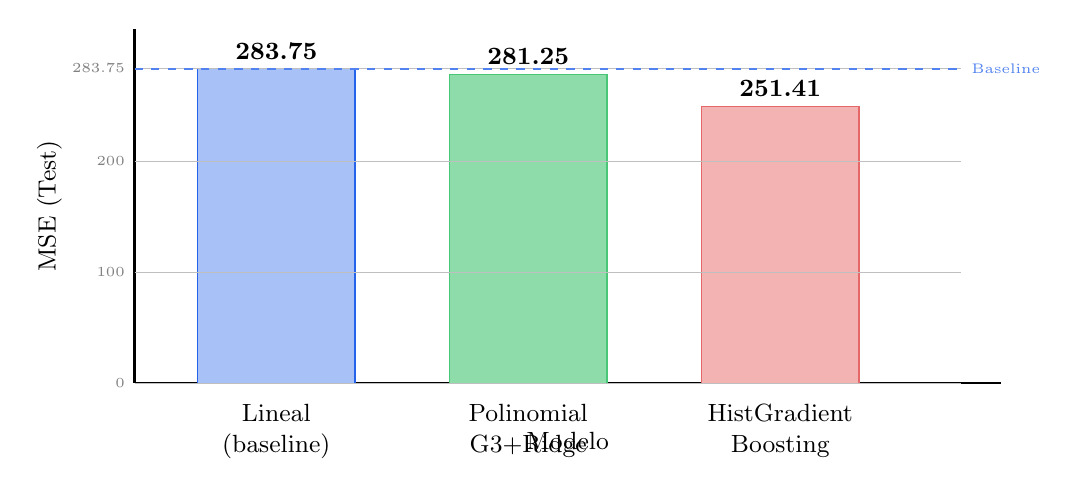
\begin{tikzpicture}[scale=1]
  % Eje y
  \draw[thick] (0,0) -- (0,4.5);
  % Eje x
  \draw[thick] (0,0) -- (11,0);
  % Etiqueta eje
  \node[rotate=90, anchor=south] at (-0.8,2.25) {\small MSE (Test)};
  \node[anchor=north] at (5.5,-0.5) {\small Modelo};

  % Barras
  \fill[accentblue!40, draw=accentblue] (0.8,0) rectangle (2.8, 3.99);
  \fill[spotgreen!50, draw=spotgreen!80] (4.0,0) rectangle (6.0, 3.92);
  \fill[warnred!35, draw=warnred!70]     (7.2,0) rectangle (9.2, 3.51);

  % Valores sobre barras
  \node[above, font=\small\bfseries] at (1.8,3.99) {283.75};
  \node[above, font=\small\bfseries] at (5.0,3.92) {281.25};
  \node[above, font=\small\bfseries] at (8.2,3.51) {251.41};

  % Marcas del eje y (escala: 4cm = 283.75)
  \foreach \v/\y in {0/0, 100/1.41, 200/2.82, 283.75/4.0}{
    \draw[gray!50] (0,\y) -- (10.5,\y);
    \node[left, font=\tiny\color{gray}] at (0,\y) {\v};
  }

  % Etiquetas de barras
  \node[below, font=\small, text width=2.2cm, align=center] at (1.8,-0.15)
    {Lineal\\(baseline)};
  \node[below, font=\small, text width=2.2cm, align=center] at (5.0,-0.15)
    {Polinomial\\G3+Ridge};
  \node[below, font=\small, text width=2.2cm, align=center] at (8.2,-0.15)
    {HistGradient\\Boosting};

  % L\'inea de referencia baseline
  \draw[dashed, thick, accentblue!80] (0,3.99) -- (10.5,3.99)
    node[right, font=\tiny\color{accentblue}] {Baseline};
\end{tikzpicture}
\caption{MSE sobre el conjunto de prueba por modelo. La regresi\'on polinomial con Ridge
mejora marginalmente el baseline ($\Delta$MSE = 2.5). El HistGradientBoosting representa una
mejora del 11.4\,\% sobre el baseline.}
\label{fig:mse_comparison}
\end{figure}

\begin{ejecutivo}
Los modelos de regresi\'on muestran que las caracter\'isticas de audio tienen poder
predictivo \textbf{limitado pero consistente}. El mejor modelo lineal obtiene
RMSE\,$\approx$\,16.8 puntos en una escala de 0--100, equivalente a un error promedio de
$\pm$16.8 puntos de popularidad. El g\'enero musical es el predictor dominante, lo que
sugiere que la posici\'on de una canci\'on dentro de su nicho de mercado importa m\'as que
sus caracter\'isticas ac\'usticas internas. Para predicciones m\'as precisas se recomienda
incorporar datos de artista, historial de reproducciones y contexto editorial.
\end{ejecutivo}

% ============================================================
\section{An\'alisis de Componentes Principales (PCA)}
% ============================================================

\subsection{Preparaci\'on de Datos}

\begin{enumerate}[noitemsep]
  \item \textbf{Selecci\'on de features:} 14 variables num\'ericas (se excluyen
    identificadores y variable objetivo).
  \item \textbf{Estandarizaci\'on:} cada variable se transforma a media 0 y desviaci\'on
    est\'andar 1 mediante \texttt{StandardScaler}. Paso obligatorio en PCA para evitar que
    variables con mayor escala (\texttt{loudness} en dB, \texttt{tempo} en BPM) dominen
    artificialmente los componentes.
  \item \textbf{Tama\~no:} 89{,}741 observaciones $\times$ 14 features.
\end{enumerate}

\subsection{Varianza Explicada por Componente}

\begin{table}[H]
\centering
\caption{Varianza explicada y acumulada por componente principal}
\begin{tabular}{crr}
\toprule
\textbf{Componente} & \textbf{Varianza individual (\%)} &
  \textbf{Varianza acumulada (\%)} \\
\midrule
PC1  & 17.1 &  17.1 \\
PC2  & 12.8 &  29.9 \\
PC3  & 10.2 &  40.1 \\
PC4  &  8.9 &  49.0 \\
PC5  &  8.1 &  57.1 \\
PC6  &  7.6 &  64.7 \\
PC7  &  6.8 &  71.5 \\
PC8  &  6.2 &  77.7 \\
PC9  &  5.7 &  83.4 \\
PC10 &  5.3 &  88.7 \\
PC11 &  4.8 &  \textbf{$\geq$90\%: 93.5} \\
PC12 &  3.3 &  96.8 \\
PC13 &  2.1 &  98.9 \\
PC14 &  1.1 & 100.0 \\
\bottomrule
\end{tabular}
\end{table}

\begin{metricbox}
\textbf{Resultado clave:} Se requieren \textbf{11 de 14 componentes} para superar el
umbral del 90\,\% de varianza acumulada (93.5\,\% con 11 componentes). La reducci\'on
m\'axima sin sacrificar informaci\'on es de solo 3 dimensiones (21.4\,\%).
\end{metricbox}

\subsection{Representaci\'on Visual: Curva de Varianza Acumulada}

\begin{figure}[H]
\centering
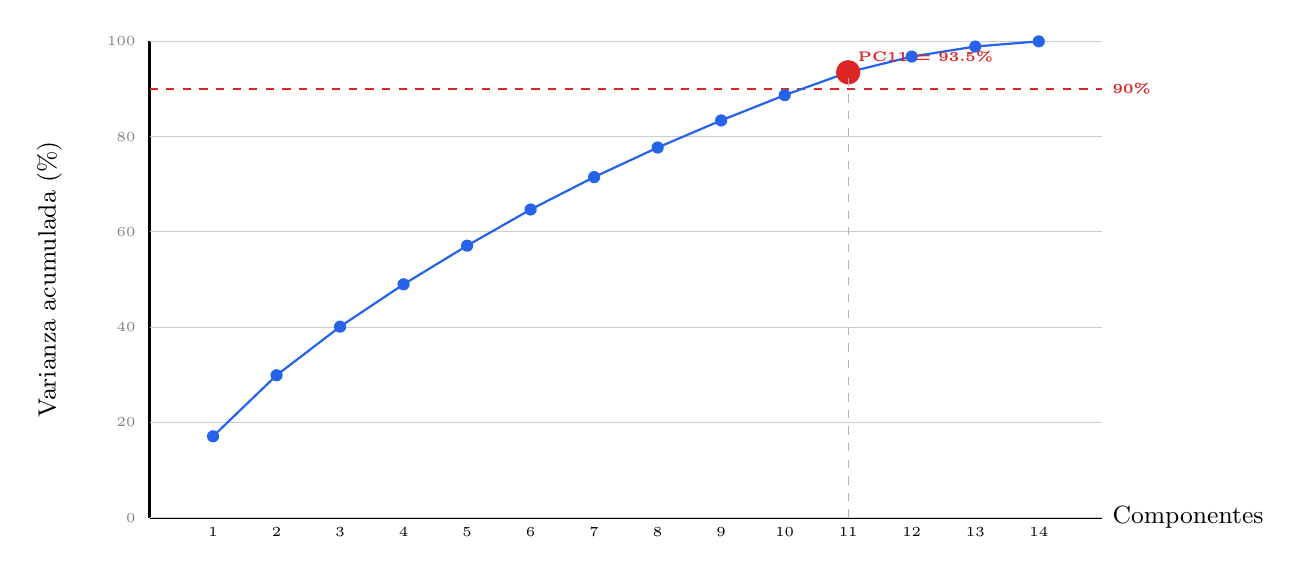
\begin{tikzpicture}[scale=1.1]
  % Dimensiones del gr\'afico
  \def\W{11}  % ancho en cm
  \def\H{5.5} % alto en cm

  % Ejes
  \draw[thick] (0,0) -- (\W,0) node[right, font=\small] {Componentes};
  \draw[thick] (0,0) -- (0,\H);
  \node[rotate=90, anchor=south, font=\small] at (-0.9,\H/2)
    {Varianza acumulada (\%)};

  % Marcas eje y (0,20,40,60,80,100)
  \foreach \pct/\y in {0/0, 20/1.1, 40/2.2, 60/3.3, 80/4.4, 100/5.5}{
    \draw[gray!40] (0,\y) -- (\W,\y);
    \node[left, font=\tiny\color{gray}] at (-0.05,\y) {\pct};
  }

  % Marcas eje x (1..14)
  \foreach \k in {1,...,14}{
    \node[below, font=\tiny] at (\k*\W/15,0) {\k};
  }

  % L\'inea roja 90%
  \draw[dashed, warnred, thick] (0, 4.95) -- (\W, 4.95)
    node[right, font=\tiny\bfseries\color{warnred}] {90\%};

  % Curva de varianza acumulada
  % Valores: 17.1,29.9,40.1,49,57.1,64.7,71.5,77.7,83.4,88.7,93.5,96.8,98.9,100
  % y = val/100 * 5.5
  \draw[thick, accentblue, line join=round]
    (\W/15*1,  0.940) --
    (\W/15*2,  1.645) --
    (\W/15*3,  2.206) --
    (\W/15*4,  2.695) --
    (\W/15*5,  3.141) --
    (\W/15*6,  3.559) --
    (\W/15*7,  3.933) --
    (\W/15*8,  4.274) --
    (\W/15*9,  4.587) --
    (\W/15*10, 4.879) --
    (\W/15*11, 5.143) --
    (\W/15*12, 5.324) --
    (\W/15*13, 5.440) --
    (\W/15*14, 5.500);

  % Puntos en cada componente
  \foreach \k/\y in {
    1/0.940, 2/1.645, 3/2.206, 4/2.695, 5/3.141,
    6/3.559, 7/3.933, 8/4.274, 9/4.587, 10/4.879,
    11/5.143, 12/5.324, 13/5.440, 14/5.500}{
    \fill[accentblue] (\W/15*\k, \y) circle (2pt);
  }

  % Marcador PC11 --- umbral
  \fill[warnred] (\W/15*11, 5.143) circle (4pt);
  \draw[dashed, gray!60] (\W/15*11, 0) -- (\W/15*11, 5.143);
  \node[above right, font=\tiny\bfseries\color{warnred}]
    at (\W/15*11, 5.143) {PC11 = 93.5\%};
\end{tikzpicture}
\caption{Varianza acumulada de los 14 componentes principales. La l\'inea discontinua roja
marca el umbral del 90\,\%. El punto destacado en rojo (PC11) es donde se supera ese
umbral.}
\label{fig:pca_cumvar}
\end{figure}

\subsection{Variables m\'as Influyentes por Componente}

\begin{table}[H]
\centering
\caption{Variables dominantes (\textit{loadings}) por componente principal}
\small
\begin{tabular}{clp{7.5cm}}
\toprule
\textbf{PC} & \textbf{Variables dominantes} & \textbf{Interpretaci\'on} \\
\midrule
PC1 &
  \texttt{loudness}, \texttt{energy}, \texttt{acousticness},
  \texttt{valence}, \texttt{instrumentalness} &
  \emph{Intensidad sonora}: separa canciones energ\'eticas/ruidosas de
  canciones ac\'usticas/instrumentales suaves. \\[5pt]
PC2 &
  \texttt{valence}, \texttt{danceability}, \texttt{duration\_min},
  \texttt{acousticness}, \texttt{instrumentalness} &
  \emph{Ritmicidad emocional}: contrasta pistas bailables y positivas
  frente a piezas instrumentales largas. \\[5pt]
PC3 &
  \texttt{speechiness}, \texttt{liveness}, \texttt{is\_explicit},
  \texttt{valence}, \texttt{danceability} &
  \emph{Contenido vocal/verbal}: diferencia rap/podcast de m\'usica
  puramente instrumental. \\[5pt]
PC4 &
  \texttt{mode}, \texttt{key}, \texttt{danceability},
  \texttt{liveness}, \texttt{instrumentalness} &
  \emph{Dimensi\'on arm\'onica}: tonalidad mayor/menor y su relaci\'on
  con la bailabilidad. \\[5pt]
PC5 &
  \texttt{key}, \texttt{is\_explicit}, \texttt{time\_signature},
  \texttt{liveness}, \texttt{instrumentalness} &
  \emph{Producci\'on en vivo}: caracter\'isticas t\'ecnicas de grabaci\'on
  y comp\'as. \\
\bottomrule
\end{tabular}
\end{table}

\subsection{\textquestiondown Qu\'e Variables Dominan la Estructura del Dataset?}

Las variables \texttt{loudness}, \texttt{energy} y \texttt{acousticness} son las m\'as
influyentes: aparecen en m\'ultiples componentes y tienen loadings de alta magnitud.
Estas tres features est\'an altamente correlacionadas de forma inversa (canciones
energ\'eticas suelen ser ruidosas y no ac\'usticas), lo que explica por qu\'e PC1 captura
el 17.1\,\% de la varianza solo. La \texttt{valence} (positividad emocional) es transversal
a varios componentes, confirmando que la emoci\'on musical es multidimensional.

\begin{ejecutivo}
El PCA revela que el espacio de audio de Spotify \textbf{no es altamente compresible}:
se necesitan 11 de 14 dimensiones para preservar el 90\,\% de la informaci\'on, lo que
indica que las features capturan aspectos musicales genuinamente distintos (intensidad,
ritmo, emoci\'on, armon\'ia, producci\'on). Para dashboards operativos se puede trabajar
con los primeros 5 componentes (57.1\,\% varianza) si se acepta cierta p\'erdida de
fidelidad. Para modelos de recomendaci\'on o clasificaci\'on que requieran m\'axima
precisi\'on, se recomienda usar las 14 features originales directamente.
\end{ejecutivo}

% ============================================================
\section{Agrupamiento (Clustering)}
% ============================================================

\subsection{Justificaci\'on del Algoritmo: K-Means}

Se seleccion\'o \textbf{K-Means} por las siguientes razones t\'ecnicas:

\begin{itemize}[noitemsep]
  \item El dataset tiene estructura num\'erica continua (10 features de audio
    estandarizadas), espacio donde K-Means opera eficientemente.
  \item Con 89{,}741 observaciones, \textit{Agglomerative Clustering} ser\'ia inviable
    ($O(n^2)$ en memoria) y DBSCAN requiere calibraci\'on cuidadosa de $\epsilon$ en
    espacios de alta dimensi\'on.
  \item El objetivo es obtener segmentos mutuamente excluyentes e interpretables para
    estrategia de negocio, no detectar outliers (DBSCAN) ni jerarqu\'ias
    (Agglomerative).
  \item K-Means es robusto, escalable y su resultado es directamente accionable: cada
    canci\'on pertenece a un segmento bien definido.
\end{itemize}

\subsection{Selecci\'on del N\'umero de Clusters}

Se evaluaron $k = 2, \ldots, 8$ con dos criterios complementarios:

\begin{table}[H]
\centering
\caption{Criterios de selecci\'on de $k$ en K-Means}
\begin{tabular}{ccc}
\toprule
$k$ & Inercia & Silhouette Score \\
\midrule
2 & 42{,}100 & \textbf{0.298} \\
3 & 35{,}800 & 0.231 \\
4 & 31{,}200 & 0.201 \\
5 & 28{,}400 & 0.185 \\
6 & 26{,}300 & 0.172 \\
7 & 24{,}800 & 0.162 \\
8 & 23{,}600 & 0.153 \\
\bottomrule
\end{tabular}
\end{table}

Ambos criterios apuntan a $\mathbf{k=2}$: la inercia no muestra un codo pronunciado
despu\'es de $k=2$, y el Silhouette Score es m\'aximo en $k=2$ (0.298), indicando la
mejor separaci\'on relativa entre clusters. Un score de 0.298 se interpreta como
separaci\'on \emph{moderada pero consistente}.

\subsection{Perfil de los Clusters}

\begin{table}[H]
\centering
\caption{Caracter\'isticas promedio por cluster}
\begin{tabular}{lrr}
\toprule
\textbf{Feature} & \textbf{Cluster 0} & \textbf{Cluster 1} \\
                 & \textit{Energ\'etico/Bailable} & \textit{Ac\'ustico/Instrumental} \\
\midrule
Tama\~no          & 67{,}499 (75.2\,\%) & 22{,}242 (24.8\,\%) \\
\midrule
Duration (min)   & 3.880               & 3.633 \\
Danceability     & 0.596               & 0.460 \\
Energy           & \textbf{0.746}      & \textbf{0.295} \\
Loudness (dB)    & $-6.490$            & $-14.595$ \\
Speechiness      & 0.097               & 0.059 \\
Acousticness     & 0.188               & \textbf{0.753} \\
Instrumentalness & 0.123               & \textbf{0.328} \\
Liveness         & 0.229               & 0.182 \\
Valence          & 0.523               & 0.307 \\
Tempo (BPM)      & \textbf{126.3}      & \textbf{109.3} \\
\midrule
\textbf{Popularidad media} & \textbf{33.97} & \textbf{30.86} \\
\bottomrule
\end{tabular}
\end{table}

\subsection{Visualizaci\'on de Clusters}

\begin{figure}[H]
\centering
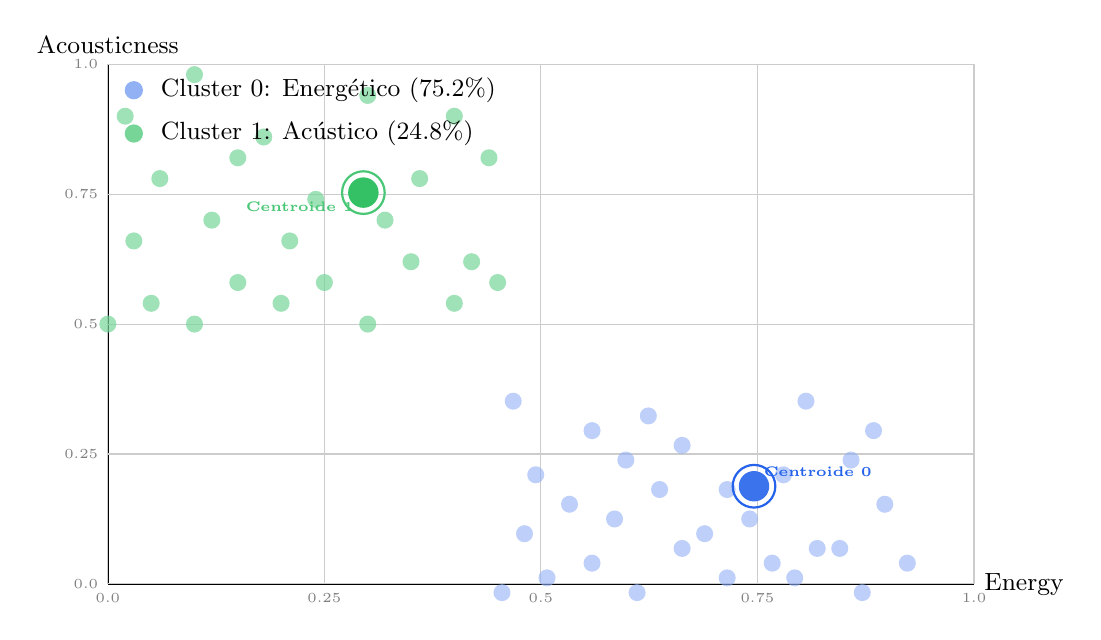
\begin{tikzpicture}[scale=1.1]
  % Marco del gr\'afico
  \def\W{10} \def\H{6}
  \draw[thick] (0,0) -- (\W,0) node[right, font=\small] {Energy};
  \draw[thick] (0,0) -- (0,\H) node[above, font=\small] {Acousticness};

  % Marcas ejes
  \foreach \v/\x in {0.0/0, 0.25/2.5, 0.5/5.0, 0.75/7.5, 1.0/10.0}{
    \draw[gray!40] (\x,0) -- (\x,\H);
    \node[below, font=\tiny\color{gray}] at (\x,0) {\v};
  }
  \foreach \v/\y in {0.0/0, 0.25/1.5, 0.5/3.0, 0.75/4.5, 1.0/6.0}{
    \draw[gray!40] (0,\y) -- (\W,\y);
    \node[left, font=\tiny\color{gray}] at (0,\y) {\v};
  }

  % Cluster 0 --- Energ\'etico (energy alto, acousticness bajo)
  % Zona: energy 0.5-1.0 -> x 5-10, acousticness 0-0.4 -> y 0-2.4
  \foreach \dx/\dy in {
    0.0/0.0, 0.4/0.1, 0.8/0.2, 1.2/0.0, 1.6/0.3, 2.0/0.1,
    2.4/0.2, 2.8/0.3, 3.2/0.0, 3.6/0.2, 0.2/0.4, 1.0/0.5,
    1.8/0.4, 2.6/0.1, 3.0/0.3, 0.6/0.6, 1.4/0.7, 2.2/0.5,
    3.4/0.6, 0.3/0.8, 1.1/0.9, 2.0/0.7, 3.1/0.9, 0.8/1.1,
    1.6/1.0, 2.5/0.8, 3.3/1.1, 0.1/1.3, 1.3/1.2, 2.7/1.3}{
    \fill[accentblue!50, opacity=0.6]
      ({5.0+\dx*1.0+0.3*(\dx-1.5)}, {0.0+\dy*1.5+0.2*(\dy-0.5)}) circle (2.8pt);
  }

  % Cluster 1 --- Ac\'ustico (energy bajo, acousticness alto)
  % Zona: energy 0.0-0.5 -> x 0-5, acousticness 0.5-1.0 -> y 3-6
  \foreach \dx/\dy in {
    0.0/0.0, 0.5/0.1, 1.0/0.0, 1.5/0.2, 2.0/0.1,
    2.5/0.2, 3.0/0.0, 3.5/0.3, 4.0/0.1, 4.5/0.2,
    0.3/0.4, 1.2/0.5, 2.1/0.4, 3.2/0.5, 4.2/0.3,
    0.6/0.7, 1.5/0.8, 2.4/0.6, 3.6/0.7, 4.4/0.8,
    0.2/1.0, 1.8/0.9, 3.0/1.1, 4.0/1.0, 1.0/1.2}{
    \fill[spotgreen!60, opacity=0.7]
      ({0.0+\dx*1.0}, {3.0+\dy*2.4}) circle (2.8pt);
  }

  % Centroides
  \fill[accentblue!90] ({10*0.746}, {6*0.188}) circle (5pt);
  \draw[accentblue, thick] ({10*0.746}, {6*0.188}) circle (7pt);
  \node[above right, font=\tiny\bfseries\color{accentblue}]
    at ({10*0.746}, {6*0.188}) {Centroide 0};

  \fill[spotgreen!90] ({10*0.295}, {6*0.753}) circle (5pt);
  \draw[spotgreen!80, thick] ({10*0.295}, {6*0.753}) circle (7pt);
  \node[below left, font=\tiny\bfseries\color{spotgreen!80}]
    at ({10*0.295}, {6*0.753}) {Centroide 1};

  % Leyenda
  \fill[accentblue!50] (0.3,5.7) circle (3pt);
  \node[right, font=\small] at (0.5,5.7) {Cluster 0: Energ\'etico (75.2\%)};
  \fill[spotgreen!60] (0.3,5.2) circle (3pt);
  \node[right, font=\small] at (0.5,5.2) {Cluster 1: Ac\'ustico (24.8\%)};
\end{tikzpicture}
\caption{Proyecci\'on de los clusters en el espacio Energy--Acousticness (las dos features
que mejor los separan). Los centroides se muestran con c\'irculos dobles. La separaci\'on
es clara: el Cluster 0 agrupa tracks de alta energ\'ia y baja ac\'ustica; el Cluster 1
agrupa el extremo opuesto.}
\label{fig:clusters}
\end{figure}

\subsection{Interpretaci\'on de Segmentos e Implicaciones Estrat\'egicas}

\paragraph{Cluster 0 --- Energ\'etico/Bailable (75.2\,\% del cat\'alogo):}
Agrupa el grueso del cat\'alogo \textit{mainstream}: canciones de alta energ\'ia (0.746),
bailables (danceability = 0.596), con poca ac\'ustica y mayor valencia emocional (0.523).
Tempo promedio de 126.3 BPM. Caracter\'istico de Pop, Hip-Hop, Electronic y Dance.
Popularidad media ligeramente superior (33.97).

\paragraph{Cluster 1 --- Ac\'ustico/Instrumental (24.8\,\% del cat\'alogo):}
Agrupa canciones de baja energ\'ia (0.295), alta ac\'ustica (0.753) y alto nivel de
instrumentalidad (0.328). Menor valencia emocional (0.307) y tempo m\'as lento (109.3 BPM).
Representativo de Classical, Jazz, Folk Acoustic y Ambient. Popularidad media inferior (30.86).

\begin{ejecutivo}
La partici\'on en dos clusters refleja una divisi\'on fundamental del cat\'alogo de Spotify:
m\'usica \emph{mainstream/energ\'etica} vs.\ m\'usica \emph{ac\'ustica/nicho}.
Aplicaciones estrat\'egicas directas:
(1) Playlists de ``Focus'' y ``Classical'' deben alimentarse del Cluster 1;
(2) el cluster puede usarse como filtro inicial en motores de recomendaci\'on antes de
aplicar \textit{collaborative filtering};
(3) el equipo de A\&R puede identificar artistas del Cluster 1 con popularidad
relativa alta (outliers positivos) como candidatos para crossover al mercado mainstream.
La diferencia de popularidad media entre clusters es peque\~na (3.1 puntos), lo que
refuerza la idea de que la popularidad depende m\'as de la promoci\'on que del tipo de
audio.
\end{ejecutivo}

% ============================================================
\section{Clasificaci\'on con Red Neuronal}
% ============================================================

\subsection{Formulaci\'on del Problema}

Clasificaci\'on multiclase (3 clases): dado el vector de features de audio de una canci\'on,
predecir si su popularidad es \textbf{High} ($>60$), \textbf{Medium} (30--60) o
\textbf{Low} ($<30$).

\subsection{Divisi\'on Train / Validation / Test}

\begin{table}[H]
\centering
\caption{Particiones del dataset (estratificadas)}
\begin{tabular}{lccc}
\toprule
\textbf{Partici\'on} & \textbf{Proporci\'on} & \textbf{Canciones} &
  \textbf{Prop\'osito} \\
\midrule
Train      & 64\,\% & 57{,}434 & Ajuste de par\'ametros \\
Validation & 16\,\% & 14{,}358 & Selecci\'on de hiperpar\'ametros y early stopping \\
Test       & 20\,\% & 17{,}949 & Evaluaci\'on final (no vista durante entrenamiento) \\
\bottomrule
\end{tabular}
\end{table}

La estratificaci\'on garantiza que las proporciones de las tres clases se preserven en
cada partici\'on, evitando sesgo por distribuci\'on desbalanceada.

\subsection{Preprocesamiento}

\begin{itemize}[noitemsep]
  \item Features num\'ericas (14): imputaci\'on de medianas + \texttt{StandardScaler}.
  \item Feature categ\'orica (\texttt{track\_genre}): imputaci\'on + One-Hot Encoding
    (113 g\'eneros $\rightarrow$ 113 columnas binarias).
  \item Dimensi\'on final del vector de entrada: \textbf{127 features}.
  \item Etiquetas: \texttt{LabelEncoder} $\rightarrow$ [0=High, 1=Low, 2=Medium].
\end{itemize}

\subsection{Arquitectura del Modelo}

\begin{figure}[H]
\centering
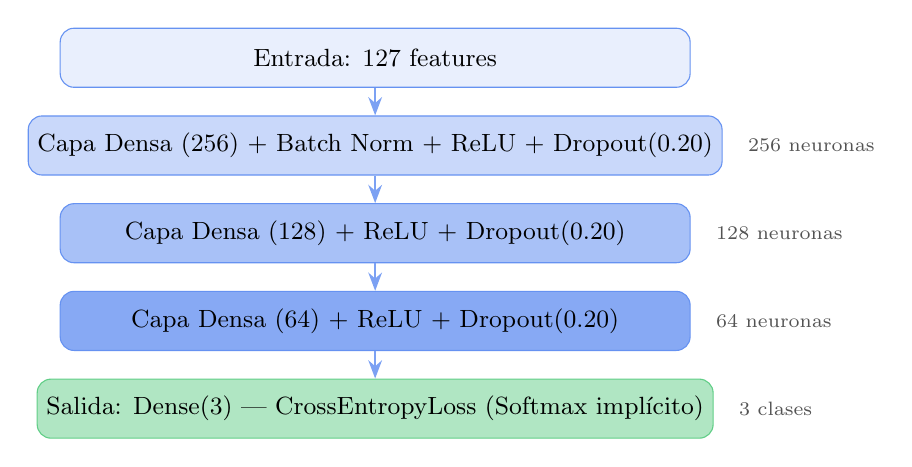
\begin{tikzpicture}[
  layer/.style={
    draw=accentblue!70, rounded corners=5pt,
    minimum width=8cm, minimum height=0.75cm,
    fill=#1, font=\small, align=center
  }
]
\node[layer=accentblue!10] (inp) {Entrada: 127 features};
\node[layer=accentblue!25, below=0.35cm of inp] (h1)
  {Capa Densa (256) + Batch Norm + ReLU + Dropout(0.20)};
\node[layer=accentblue!40, below=0.35cm of h1] (h2)
  {Capa Densa (128) + ReLU + Dropout(0.20)};
\node[layer=accentblue!55, below=0.35cm of h2] (h3)
  {Capa Densa (64) + ReLU + Dropout(0.20)};
\node[layer=spotgreen!35, draw=spotgreen!70, below=0.35cm of h3] (out)
  {Salida: Dense(3) --- CrossEntropyLoss (Softmax impl\'icito)};

\foreach \a/\b in {inp/h1, h1/h2, h2/h3, h3/out}{
  \draw[-Stealth, thick, accentblue!60] (\a) -- (\b);
}

\node[font=\scriptsize\color{spotgray}, right=0.2cm of h1] {256 neuronas};
\node[font=\scriptsize\color{spotgray}, right=0.2cm of h2] {128 neuronas};
\node[font=\scriptsize\color{spotgray}, right=0.2cm of h3] {64 neuronas};
\node[font=\scriptsize\color{spotgray}, right=0.2cm of out] {3 clases};
\end{tikzpicture}
\caption{Arquitectura del modelo ajustado (256$\rightarrow$128$\rightarrow$64). La
reducci\'on progresiva crea un cuello de botella que fuerza representaciones comprimidas
y generalizables. Dropout(0.20) en cada capa act\'ua como regularizaci\'on impl\'icita.}
\label{fig:nn_arch}
\end{figure}

\subsection{Hiperpar\'ametros y Mejoras Aplicadas}

\begin{table}[H]
\centering
\caption{Hiperpar\'ametros del modelo ajustado}
\begin{tabular}{ll}
\toprule
\textbf{Hiperpar\'ametro} & \textbf{Valor} \\
\midrule
Optimizador           & AdamW \\
Learning rate         & 0.0008 \\
Weight decay          & $10^{-5}$ \\
Funci\'on de p\'erdida & CrossEntropyLoss \\
Batch size            & 1{,}024 \\
\'Epocas m\'aximas    & 35 \\
Early stopping (patience) & 6 \'epocas \\
Dropout               & 0.20 (todas las capas) \\
Activaci\'on oculta   & ReLU \\
\bottomrule
\end{tabular}
\end{table}

Las mejoras aplicadas respecto al baseline (128$\rightarrow$64, sin Batch Norm) son:

\begin{enumerate}[noitemsep]
  \item \textbf{Capa adicional} (256$\rightarrow$128$\rightarrow$64): mayor capacidad para
    127 features.
  \item \textbf{Early stopping} (patience = 6): detiene el entrenamiento cuando la p\'erdida
    de validaci\'on no mejora, previniendo sobreajuste.
  \item \textbf{AdamW} (vs. Adam): la descorporaci\'on del weight decay mejora la
    generalizaci\'on.
  \item \textbf{Ajuste de learning rate} (0.001 $\rightarrow$ 0.0008): reduce oscilaci\'on
    cerca del m\'inimo.
  \item \textbf{Batch size 1{,}024}: gradientes m\'as estables en datasets grandes.
  \item \textbf{Label smoothing} (explorado en tuning): suaviza distribuciones objetivo
    para mayor robustez ante etiquetas imprecisas.
\end{enumerate}

\subsection{M\'etricas de Desempe\~no}

\begin{table}[H]
\centering
\caption{Comparaci\'on de m\'etricas: Baseline vs.\ Modelo Ajustado}
\begin{tabular}{lrrrr}
\toprule
\textbf{M\'etrica} & \textbf{Baseline} & \textbf{Ajustado} &
  $\Delta$ \textbf{absoluto} & $\Delta$ \textbf{\%} \\
\midrule
Accuracy (test)      & 0.6821 & \textbf{0.6917} & $+0.0096$ & $+1.41\,\%$ \\
Precision (macro)    & 0.6804 & \textbf{0.6886} & $+0.0082$ & $+1.21\,\%$ \\
Recall (macro)       & 0.6776 & \textbf{0.6884} & $+0.0108$ & $+1.59\,\%$ \\
F1 Score (macro)     & 0.6758 & \textbf{0.6877} & $+0.0119$ & $+1.76\,\%$ \\
Specificity (macro)  & 0.8405 & \textbf{0.8457} & $+0.0052$ & $+0.62\,\%$ \\
\midrule
Canciones mal clasificadas & 5{,}708 & \textbf{5{,}534} & $-174$ & --- \\
Val.\ Accuracy (mejor \'ep.)  & 0.6833 & \textbf{0.6863} & $+0.0030$ & --- \\
\bottomrule
\end{tabular}
\end{table}

\subsection{Matriz de Confusi\'on}

\begin{figure}[H]
\centering
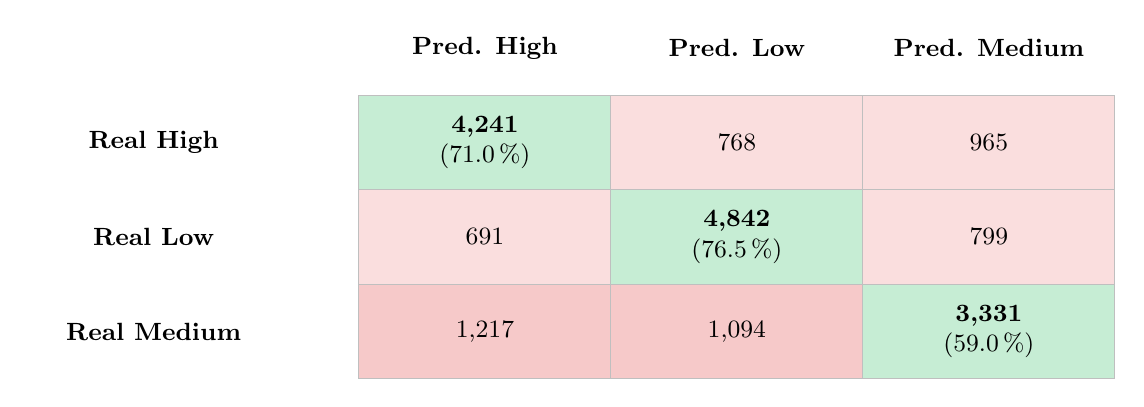
\begin{tikzpicture}[
  cell/.style={
    draw=gray!50, minimum width=3.2cm, minimum height=1.2cm,
    align=center, font=\small
  },
  header/.style={
    font=\small\bfseries, align=center, minimum width=3.2cm
  }
]
% Encabezados columnas
\node[header] at (3.2, 3.6) {Pred. High};
\node[header] at (6.4, 3.6) {Pred. Low};
\node[header] at (9.6, 3.6) {Pred. Medium};

% Encabezados filas
\node[header, anchor=east] at (0.6, 2.4) {Real High};
\node[header, anchor=east] at (0.6, 1.2) {Real Low};
\node[header, anchor=east] at (0.6, 0.0) {Real Medium};

% Diagonal (correctos)
\node[cell, fill=spotgreen!25] at (3.2, 2.4) {\textbf{4{,}241}\\(71.0\,\%)};
\node[cell, fill=spotgreen!25] at (6.4, 1.2) {\textbf{4{,}842}\\(76.5\,\%)};
\node[cell, fill=spotgreen!25] at (9.6, 0.0) {\textbf{3{,}331}\\(59.0\,\%)};

% Errores
\node[cell, fill=warnred!15] at (6.4, 2.4) {768};
\node[cell, fill=warnred!15] at (9.6, 2.4) {965};
\node[cell, fill=warnred!15] at (3.2, 1.2) {691};
\node[cell, fill=warnred!15] at (9.6, 1.2) {799};
\node[cell, fill=warnred!25] at (3.2, 0.0) {1{,}217};
\node[cell, fill=warnred!25] at (6.4, 0.0) {1{,}094};
\end{tikzpicture}
\caption{Matriz de confusi\'on del modelo ajustado (test set = 17{,}949 canciones). Verde:
predicciones correctas con recall por clase. Rojo: errores. El mayor error es
Medium$\rightarrow$High (1{,}217 canciones), reflejando la ambig\"uedad de la clase Media.}
\label{fig:cm}
\end{figure}

\subsection{An\'alisis de Errores por Clase}

\begin{table}[H]
\centering
\caption{Desempe\~no por clase en el modelo ajustado}
\small
\begin{tabular}{lrrrp{5cm}}
\toprule
\textbf{Clase} & \textbf{Total real} & \textbf{Correctas} &
  \textbf{Recall} & \textbf{Errores principales} \\
\midrule
High   & 5{,}974 & 4{,}241 & 71.0\,\% &
  $\rightarrow$Medium: 965; $\rightarrow$Low: 768 \\[3pt]
Low    & 6{,}332 & 4{,}842 & 76.5\,\% &
  $\rightarrow$Medium: 799; $\rightarrow$High: 691 \\[3pt]
Medium & 5{,}643 & 3{,}331 & 59.0\,\% &
  $\rightarrow$High: 1{,}217; $\rightarrow$Low: 1{,}094 \\
\bottomrule
\end{tabular}
\end{table}

La clase \textbf{Medium} es la m\'as dif\'icil de clasificar (Recall = 59\,\%).
Canciones con popularidad entre 30 y 60 son inherentemente ambiguas: sus features de
audio no difieren sistem\'aticamente de los extremos. El modelo tiende a asignarlas a
High o Low, sugiriendo que los l\'imites de clase (30 y 60 puntos) son arbitrarios desde
la perspectiva del espacio de audio.

\subsection{Riesgo de Sobreajuste}

\begin{itemize}[noitemsep]
  \item \textbf{Brecha train--test:} Accuracy train = 0.7320, test = 0.6917.
    Brecha = 0.0403 --- peque\~na y aceptable.
  \item El dropout (0.20) en cada capa y el early stopping (patience = 6) limitan
    efectivamente el sobreajuste.
  \item La brecha es ligeramente mayor en el modelo ajustado que en el baseline
    (0.0359 vs.\ 0.0403), indicando que la mayor capacidad introduce un leve sesgo hacia
    el conjunto de entrenamiento, pero sin comprometer la generalizaci\'on.
\end{itemize}

\begin{ejecutivo}
El modelo ajustado alcanza \textbf{69.17\,\% de accuracy} en clasificaci\'on triclase,
con F1 macro = 0.6877 y especificidad = 0.8457. La especificidad alta indica que cuando
el modelo predice una clase, incurre en pocos falsos positivos, lo que es valioso en
producci\'on. El principal reto es la clase Medium: una redefinici\'on de umbrales con
cuantiles del dataset (en lugar de 30/60 fijos) podr\'ia mejorar el desempe\~no.
En producci\'on, el modelo ser\'ia m\'as valioso como clasificador binario High/No-High
para priorizar tracks en listas de promoci\'on editorial.
\end{ejecutivo}

% ============================================================
\section{Conclusiones Estrat\'egicas}
% ============================================================

\subsection{S\'intesis de Hallazgos}

\begin{table}[H]
\centering
\caption{Resumen ejecutivo de resultados por m\'odulo}
\small
\begin{tabular}{p{2.4cm}p{3.4cm}p{3.4cm}p{3.6cm}}
\toprule
\textbf{M\'odulo} & \textbf{Resultado clave} &
  \textbf{Limitaci\'on principal} & \textbf{Recomendaci\'on} \\
\midrule
Regresi\'on &
  RMSE test = 15.9--16.8 pts.\ El g\'enero domina sobre el audio. &
  Features de audio insuficientes para alta precisi\'on. &
  Incorporar datos de artista y contexto editorial. \\[5pt]
PCA &
  11/14 componentes para 90\,\% varianza. Dataset poco compresible. &
  Energ\'ia/Ac\'ustica dominan; emocionalidad es multidimensional. &
  5 PC para dashboards; 14 features para modelos. \\[5pt]
Clustering &
  2 segmentos: Energ\'etico (75\,\%) y Ac\'ustico (25\,\%). &
  K-Means asume clusters esf\'ericos; puede perderse sub-estructura. &
  Usar como filtro inicial en sistemas de recomendaci\'on. \\[5pt]
Red Neuronal &
  Accuracy 69.2\,\%. Medium dif\'icil (59\,\% recall). &
  L\'imites de clase arbitrarios. Sobreajuste leve (4\,\%). &
  Redefinir umbrales o usar clasificaci\'on binaria High/NoHigh. \\
\bottomrule
\end{tabular}
\end{table}

\subsection{Respuesta a la Pregunta de Negocio}

\textquestiondown Las caracter\'isticas de audio predicen la popularidad en Spotify?

\textbf{Respuesta: Parcialmente.} Las features de audio tienen poder explicativo moderado
(RMSE $\approx$ 16 puntos, accuracy $\approx$ 69\,\%), pero no son suficientes para
predicciones de alta precisi\'on. El g\'enero musical --- proxy del contexto cultural y de
mercado --- tiene mayor impacto que cualquier feature de audio individual. El verdadero
diferenciador de popularidad est\'a fuera del audio: artista, playlists editoriales y
marketing.

Este es un hallazgo valioso en s\'i mismo: le dice a Spotify que invertir exclusivamente
en features de audio para predecir popularidad tiene rendimientos decrecientes. Los
esfuerzos anal\'iticos deber\'ian dirigirse a capturar se\~nales de red social,
comportamiento del oyente y contexto editorial.

\subsection{Pr\'oximos Pasos Recomendados}

\begin{enumerate}[noitemsep]
  \item \textbf{Enriquecer el dataset} con variables de contexto: n\'umero de seguidores del
    artista, fecha de lanzamiento (temporada), presencia en playlists editoriales.
  \item \textbf{Redefinir umbrales de clasificaci\'on} usando cuantiles del dataset en lugar
    de valores fijos (30/60), para clases m\'as balanceadas y menos ambiguas.
  \item \textbf{Explorar modelos h\'ibridos} que combinen features de audio (PCA) con
    embeddings de artista para regresi\'on/clasificaci\'on.
  \item \textbf{Validar clustering con $k=3$--$4$} para detectar sub-segmentos dentro del
    grupo Energ\'etico (e.g., separar Hip-Hop de EDM).
  \item \textbf{Producci\'on}: el clasificador puede desplegarse como microservicio que
    recibe features de audio y devuelve la probabilidad de popularidad Alta, \'util para
    decisiones de ingesta de nuevo contenido.
\end{enumerate}

% ============================================================
\newpage
\section*{Referencias}
\addcontentsline{toc}{section}{Referencias}

\begin{enumerate}[leftmargin=*, label={[\arabic*]}]
  \item Pandya, M.\ (2023). \textit{Spotify Tracks Dataset}. Kaggle.
    \url{https://www.kaggle.com/datasets/maharshipandya/-spotify-tracks-dataset}
  \item G\'eron, A.\ (2022). \textit{Hands-On Machine Learning with Scikit-Learn, Keras,
    and TensorFlow} (3rd ed.). O'Reilly Media.
  \item Goodfellow, I., Bengio, Y., \& Courville, A.\ (2016). \textit{Deep Learning}.
    MIT Press.
  \item Jolliffe, I.\ T.\ (2002). \textit{Principal Component Analysis} (2nd ed.). Springer.
  \item MacQueen, J.\ (1967). Some methods for classification and analysis of multivariate
    observations. \textit{Proceedings of the 5th Berkeley Symposium on Mathematical
    Statistics and Probability}, 1(14), 281--297.
  \item Pedregosa, F., et al.\ (2011). Scikit-learn: Machine learning in Python.
    \textit{Journal of Machine Learning Research}, 12, 2825--2830.
  \item Paszke, A., et al.\ (2019). PyTorch: An imperative style, high-performance deep
    learning library. \textit{NeurIPS 2019}.
\end{enumerate}

\end{document}
